\documentclass[a4paper,10pt]{article}

\usepackage{doc/header}

\begin{document}
\title{Asynchronous Server-Side Resolution Monitoring}
\author{Jason Cairns}
\year=2020 \month=9 \day=24
\maketitle{}

\section{Introduction}

The advantages of asynchrony in the system come with significant costs, with an
example of a race condition arising from asynchrony examined in
\href{ini-distobj-exp.pdf}{Initial Distributed Object Experiments}.
The correctness of this system is not altered by asynchrony in itself, but the
object models and the state of resolution in particular are clear derivatives
of errors.
In the general case, every message containing a list of distributed references
for arguments contains the implicit dependency on the resolution of those
distributed arguments which must be forced prior to emerging and aligning them
as part of standard server operations.
When unresolved references are sent through to a node that can only resolve
them after evaluating the current message, rather than being able to rely on
another node for generating a resolution, a deadlock situation arises.
This document shows some potential solutions to the issues associated with the
model in asynchronous flow.

\section{Alternating Recursive Blocking Pop and Evaluation}
\label{recurs-stack}
Rather than blocking and waiting for resolution of distributed references, an
alternative model recurses on the \mintinline{r}{server} function upon
encountering unresolved references, returning upon an evaluation which possibly
serves to resolve the relevant distributed reference.
Given that resolution dependencies form a directed acyclic graph, due to
references only being created out of existing references, and assuming a fixed
set of messages, any unresolved reference that leads to recursion will
eventually be resolved upon evaluation of it's associated message by either
another node, or more importantly, by the same node at some deeper level of
recursion.
This solution uses the call stack as a central data structure.
It is equivalent to performing a blocking pop on the message queues, then
pushing the message on a stack, and either evaluating the content of the
message or returning to the message queues, depending on whether the references
in the message are in the state of being resolved or not, respectively.

Potential for a problem arises when a node is at some recursive step, having
unresolved references, and is in the state of waiting on the message queues.
if the references contained on the node's stack all depend on jobs that are
evaluated by other nodes, thereby being marked for resolution themselves, and
no more messages come through in any of the monitored queues, the server is in
a state of having the messages on the stack ready for evaluation, yet it will
instead stay listening on it's queues indefinitely, never terminating.

This issue can be weakened by changing the pop of the message queues to be
non-blocking.
With this in place, given a message with unresolved references, a server would
recurse, perform a pop on the message queues, and either receive an element,
and perform as previously specified, or receive no element and return to check
if the message has references resolved yet, repeating the process until
resolution of the original message has taken place, thereby ideally servicing
every message that arrives to the node.

The stack data structure serves to limit even this change, in association with
the fact that popped message queues have no ordering defined between them, with
such an ordering having no means of imposition.
An example of non-termination can be given by constructing a directed acyclic
graph of dependencies, then having the stack filled in such a manner that the
ability to move to a state of evaluation is impossible.
This is given in the diagram of dependencies in figure \ref{fig:deps}, and the
stack diagram in figure \ref{fig:deps-block-stack}.

\begin{figure}
	\centering
	\begin{tikzpicture}
		\node[node] (d) {\(d\)};
		\node[node,right=of d] (c) {\(c\)};
		\node[node,right=of c] (b) {\(b\)};
		\node[node,right=of b] (a) {\(a\)};

		\begin{pgfonlayer}{categories}
			\node[category,fit=(b)(c)(d),label={Node \(A\)}] (nodea) {};
			\node[category,fit=(a),label={Node \(B\)}] (nodeb) {};
		\end{pgfonlayer}{categories}

		\draw[mypath] (d) -- (c);
		\draw[mypath] (c) -- (b);
		\draw[mypath] (b) -- (a);
	\end{tikzpicture}
	\caption{\label{fig:deps}DAG of dependencies, with arcs indicating
	direction of dependence.}
\end{figure}

\begin{figure}
	\centering
	\begin{tikzpicture}
		\startframe
		\cell{Evaluating reference: \(d\)}
		\cell{Prerequisite evaluation: \(c\)}
		\finishframe{\texttt{server()}}
		\startframe
		\cell{Evaluating reference: \(b\)}
		\cell{Prerequisite evaluation: \(a\)}
		\finishframe{\texttt{server()}}
		\startframe
		\cell{Evaluating reference: \(c\)}
		\cell{Prerequisite evaluation: \(b\)}
		\finishframe{\texttt{server()}}
		\stackbottom{}
	\end{tikzpicture}
	\caption{\label{fig:deps-block-stack}Stack causing non-termination if
	no further messages are sent under the weak recursive model.} 
\end{figure}

As can be seen, some message identified in the figure by \(d\) depends on the
evaluation of message \(c\) for resolution, but is barred from it by message
\(b\), which depends on message \(a\), which in turn is evaluated on some other
node.
The order of events in the system follow that message \(a\) is sent out by some
client, taking a very long time to be evaluated on node \(B\).
Immediately after sending, and concurrent to evaluation, messages \(b\), \(c\)
and \(d\) are sent out by the same client, and read by node \(A\) in inverse
order, as \(c\), \(b\), and \(d\).
If no more messages are sent, the end result is a constant switching between
monitoring message queues, and checking the prerequisites of message \(d\) as
to whether \(c\) has been evaluated yet, which as long as node \(A\) remains in
these described states, will never occur.

\section{Inbox List Controlling Finite State Machine}
\label{inbox-list}

The example issue given in section \ref{recurs-stack} is intrinsic to the use
of the call stack as a data structure.
Were this to be replaced with an alternative, such as a list, ideally circular,
there is the potential for overcoming the problem.
For example, if popped messages were placed on a list and paired with an
associated procedure which iterates along them, checking their resolution
status and evaluating if possible, returning eventually to read the queues,
then assuming finite messages, there will be no issues as in section
\ref{recurs-stack}.
Server pseudocode is given in listing \ref{src:q-state}, with the associated
state transition diagram in figure \ref{fig:q-state}.

\begin{srcclrs}
\begin{codebox}
	\Procname{\proc{Server}()}
	\li \(\id{inbox} \gets \proc{list()}\)
	\li \(i \gets 1\)
	\li \Repeat
	\li \(n \gets \proc{Length}(\id{inbox})\)
	\li \If \(i \isequal n + 1\)
	\li \Then
	\(\id{inbox}[i] \gets \proc{Select}(\proc{Queues}(), \id{timeout}=0)\)
	\End
	\li \If \(\proc{Resolved?}(\id{inbox}[i])\)
	\li \Then
	\(\proc{Evaluate}(\id{inbox}[i])\)
	\li \(\id{inbox}[i] \gets \const{NIL}\)
	\End
	\li \(i \gets i + 1 \mod n + 1\)
	\End
\end{codebox}
	\caption{\label{src:q-state}Pseudocode for server using elements of an
	\textit{inbox} list to control program flow.}
\end{srcclrs}

\begin{figure}
	\centering
	\begin{tikzpicture}
		\node[node] (m) {\(m\)};
		\node[right=of m] (dots) {\(\dots\)};
		\node[node,right=of dots] (n) {\(n\)};
		\node[node,right=of n] (s) {\(s\)};

		\draw[mypath] (m) to[bend left] (dots);
		\draw[mypath] (dots) to[bend left] (n);
		\draw[mypath] (n) to[bend left] (s);
		\draw[mypath] (s) to[bend left] (m);
	\end{tikzpicture}
	\caption{\label{fig:q-state}States of the \texttt{server}, with nodes
	\(m \dots n\) representing resolution checking and possible evaluation
	of elements on an \textit{inbox} list, and \(s\) representing a
	non-blocking \texttt{select}.}
\end{figure}

One very obvious issue with such an approach is the huge inefficiency of
polling, which this solution relies upon.
In addition, the number of polls for checking resolution are bounded only by
the evaluation time of the relevant prerequisites, which is theoretically
unbounded - making the poll particularly inefficient.

\section{Job Completion Queues}

\begin{figure}
	\centering
	\begin{tikzpicture}
		\node[queue] (q1) {\(q1\)};
		\node[queue,below=\blockdist of q1] (dots) {\(\dots\)};
		\node[queue,below=\blockdist of dots] (qn) {\(qn\)};

		\begin{pgfonlayer}{categories}
			\node[category,fit=(q1)(dots)(qn),label={below:Resolution Queues}] (resq) {};
		\end{pgfonlayer}{categories}

		\node[queue,above=of resq] (interest) {Job Interest Queue};
		\node[queue,below=of resq] (resk) {Resolution Key};

		\begin{pgfonlayer}{units}
			\node[unit,fit=(interest)(resk),label={Distributed Information Space}] (infsp) {};
		\end{pgfonlayer}{units}

		\node[unit,right=\commdist of infsp] (server) {Server processing the job};
		\node[left=\commdist of infsp] (null) {};
		\node[unit,above=\blockdist of null] (pre) {node \texttt{pre}};
		\node[unit,below=\blockdist of null] (post) {node \texttt{post}};

		\draw[mypath,dark2-1] (pre.north) -- (interest.west)
		node[midway,anchor=south] {1};
		\draw[mypath,dark2-1] (interest.east) -- (server.north)
		node[midway,anchor=south] {2};
		\draw[mypath,dark2-1] (server) -- (q1)
		node[pos=0.4,anchor=south] {3};
		\draw[mypath,mygray] (server) -- (dots);
		\draw[mypath,mygray] (server) -- (qn);
		\draw[mypath,mygray] (server) -- (resk);
		\draw[mypath,dark2-1] (q1) -- (pre)
		node[midway,anchor=north] {4};

		\draw[mypath,dark2-2] (post) -- (interest.south)
		node[midway,anchor=south] {1};
		\draw[mypath,dark2-2] (post) -- (resk.166)
		node[midway,anchor=south] {2};
		\draw[mypath,dark2-2] (resk.west) -- (post.south) 
		node[midway,anchor=north] {3};
	\end{tikzpicture}
	\caption{\label{fig:two-part-sol}Activity between nodes and a server
	through the distributed information space, with numbering following the
	logical order of communication events for each node. The node named
	'\texttt{pre}' seeks resolution prior to processing of the job, while
	the node '\texttt{post}' seeks resolution after the job has completed
	processing.}
\end{figure}

\begin{srcclrs}
\begin{codebox}
	\Procname{\proc{Server}()}
	\li \(\id{inbox} \gets \proc{List}()\)
	\li \Repeat
	\li \(\id{msg} \gets \proc{Select}(\proc{Queues}(), \id{timeout}=\const{Inf})\)
	\li \If \(\proc{isJobMsg?}(\id{msg})\)
	\li \Then
	\(\id{inbox}[\proc{Length}(\id{inbox})+1] \gets \id{msg}\)
	\End
	\li \(\id{inbox} \gets \proc{UpdateDependencies}(\id{inbox},\id{msg})\)
	\li \(\id{inbox} \gets \proc{evalResolvedMsgs}(\id{inbox})\)
\end{codebox}
	\caption{\label{src:two-part-sol-serv}Pseudocode for server scanning
	queues for both job messages and resolution messages, and updating
	local inbox accordingly.}
\end{srcclrs}

\begin{srcclrs}
\begin{codebox}
	\Procname{\proc{ResolutionLookup}(\(\id{chunkRef}\))}
	\li \(\id{toMonitor} \gets \proc{GetReturnQueue}()\)
	\li \(\proc{PushInterest}(\id{chunkRef}, \id{toMonitor})\)
	\li \If \(\proc{CheckResKey}(\id{chunkRef})\)
	\li \Then
	\(\proc{Cleanup}()\)
	\li \(\Return 0\)
	\li \Else
	\proc{AddToResQueues}(\id{toMonitor})
	\li \(\Return 1\)
\end{codebox}
	\caption{\label{src:two-part-sol-res}Pseudocode for resolution lookup
	of references, called as part of dependency checking in
	\texttt{UpdateDependencies} of the \texttt{Server} function at listing
	\ref{src:two-part-sol-serv}. Returns the resolution status to allow
	marking of inbox items for the \texttt{evalResolvedMsgs} function.}
\end{srcclrs}

An amendment to the solution proferred in section \ref{inbox-list} is to have
the resolution status of chunks propagated to every relevant node while they
were listening to queues already.
This may take several forms.

Possibly the simplest is to have resolution queues, as clarified job queues,
associated with each chunk reference to listen to for its resolution status, if
unresolved.
A problem occurs if multiple nodes are interested in the same chunk reference's
resolution status, and one nodes' pop will result in no information reaching
the other, though a gossip-like protocol of immediately pushing the information
back on the list after popping can get around this, ensuring that all
interested parties attain the information.
This has the cost of a large number of messages moving back and forth, as well
as the forced serialisation of one node strictly popping after another, waiting
for every round-trip.

Alternatively, a two-part solution, as per figure \ref{fig:two-part-sol} and
listings \ref{src:two-part-sol-serv} and \ref{src:two-part-sol-res} for the
server and resolution lookup respectively, could be performed with all
interested nodes posting their interest to some queue, and upon resolution the
server first posts the resolution status as a key for all interested future
nodes, then pushing directly to relevant queues for all of the nodes on the
interest queue.
Resolution lookup will reflect this in first posting interest on the interest
queue, then checking for a key, before monitoring the interest queue and
performing associated cleanup afterwards.
The unusual ordering of operations as part of resolution lookup ensures
atomicity, with there being no possibility of missing either a key or a queue
on the client end, as given through the following proof:

Consider the moment a client has successfully posted interest on the interest queue.
At this point, there are two relevent states for server communication,
dependent on whether the server has posted a key or not.

If the server has not yet posted the key, then the client is guaranteed
notification via either the server posting a key just before the client scans
for one, or the server pushing to the client's queue after the server posts the
key, were the client to move past the operation of scanning for a key, prior to
the server posting one.

If the server has posted the key, the client will then pick it up as part of
the next operation.

The solution is well paired with a local inbox with tracking of dependencies
associated with messages in the inbox.
This solution ensures none of the documented race conditions, no polling
inefficiencies, and a reasonable number of messages sent.
\end{document}
